
\documentclass[12pt,halfline,a4paper,]{ouparticle}

% Packages I think are necessary for basic Rmarkdown functionality
\usepackage{hyperref}
\usepackage{graphicx}
\usepackage{listings}
\usepackage{xcolor}
\usepackage{fancyvrb}
\usepackage{framed}

% Link coloring
\hypersetup{breaklinks=true,
            bookmarks=true,
            pdfauthor={},
            pdftitle={STA4026Z Neural Network Assignment - Hitting the Wall.}
            }


%% To allow better options for figure placement
%\usepackage{float}

% Packages that are supposedly required by OUP sty file
\usepackage{amssymb, amsmath, geometry, amsfonts, verbatim, endnotes, setspace}

% use upquote if available, for straight quotes in verbatim environments
\IfFileExists{upquote.sty}{\usepackage{upquote}}{}

% Macros for dealing with affiliations, footnotes, etc.
\makeatletter
\def\Newlabel#1#2#3{\expandafter\gdef\csname #1@#2\endcsname{#3}}

\def\Ref#1#2{\@ifundefined{#1@#2}{???}{\csname #1@#2\endcsname}}

\newcommand*\samethanks[1][\value{footnote}]{\footnotemark[#1]}

\newcommand*\ifcounter[1]{%
  \ifcsname c@#1\endcsname
    \expandafter\@firstoftwo
  \else
    \expandafter\@secondoftwo
  \fi
}

\newcommand*\thanksbycode[1]{%
  \ifcounter{FNCT@#1}
    {\samethanks[\value{FNCT@#1}]}
    {\thanks{\Ref{FN}{#1}}\newcounter{FNCT@#1}\setcounter{FNCT@#1}{\value{footnote}}}
}

% Create labels for Addresses if the are given in Elsevier format

% Create labels for Footnotes if the are given in Elsevier format

% Part for setting citation format package: natbib

% Part for setting citation format package: biblatex

% Pandoc syntax highlighting
\usepackage{color}
\usepackage{fancyvrb}
\newcommand{\VerbBar}{|}
\newcommand{\VERB}{\Verb[commandchars=\\\{\}]}
\DefineVerbatimEnvironment{Highlighting}{Verbatim}{commandchars=\\\{\}}
% Add ',fontsize=\small' for more characters per line
\usepackage{framed}
\definecolor{shadecolor}{RGB}{248,248,248}
\newenvironment{Shaded}{\begin{snugshade}}{\end{snugshade}}
\newcommand{\AlertTok}[1]{\textcolor[rgb]{0.94,0.16,0.16}{#1}}
\newcommand{\AnnotationTok}[1]{\textcolor[rgb]{0.56,0.35,0.01}{\textbf{\textit{#1}}}}
\newcommand{\AttributeTok}[1]{\textcolor[rgb]{0.13,0.29,0.53}{#1}}
\newcommand{\BaseNTok}[1]{\textcolor[rgb]{0.00,0.00,0.81}{#1}}
\newcommand{\BuiltInTok}[1]{#1}
\newcommand{\CharTok}[1]{\textcolor[rgb]{0.31,0.60,0.02}{#1}}
\newcommand{\CommentTok}[1]{\textcolor[rgb]{0.56,0.35,0.01}{\textit{#1}}}
\newcommand{\CommentVarTok}[1]{\textcolor[rgb]{0.56,0.35,0.01}{\textbf{\textit{#1}}}}
\newcommand{\ConstantTok}[1]{\textcolor[rgb]{0.56,0.35,0.01}{#1}}
\newcommand{\ControlFlowTok}[1]{\textcolor[rgb]{0.13,0.29,0.53}{\textbf{#1}}}
\newcommand{\DataTypeTok}[1]{\textcolor[rgb]{0.13,0.29,0.53}{#1}}
\newcommand{\DecValTok}[1]{\textcolor[rgb]{0.00,0.00,0.81}{#1}}
\newcommand{\DocumentationTok}[1]{\textcolor[rgb]{0.56,0.35,0.01}{\textbf{\textit{#1}}}}
\newcommand{\ErrorTok}[1]{\textcolor[rgb]{0.64,0.00,0.00}{\textbf{#1}}}
\newcommand{\ExtensionTok}[1]{#1}
\newcommand{\FloatTok}[1]{\textcolor[rgb]{0.00,0.00,0.81}{#1}}
\newcommand{\FunctionTok}[1]{\textcolor[rgb]{0.13,0.29,0.53}{\textbf{#1}}}
\newcommand{\ImportTok}[1]{#1}
\newcommand{\InformationTok}[1]{\textcolor[rgb]{0.56,0.35,0.01}{\textbf{\textit{#1}}}}
\newcommand{\KeywordTok}[1]{\textcolor[rgb]{0.13,0.29,0.53}{\textbf{#1}}}
\newcommand{\NormalTok}[1]{#1}
\newcommand{\OperatorTok}[1]{\textcolor[rgb]{0.81,0.36,0.00}{\textbf{#1}}}
\newcommand{\OtherTok}[1]{\textcolor[rgb]{0.56,0.35,0.01}{#1}}
\newcommand{\PreprocessorTok}[1]{\textcolor[rgb]{0.56,0.35,0.01}{\textit{#1}}}
\newcommand{\RegionMarkerTok}[1]{#1}
\newcommand{\SpecialCharTok}[1]{\textcolor[rgb]{0.81,0.36,0.00}{\textbf{#1}}}
\newcommand{\SpecialStringTok}[1]{\textcolor[rgb]{0.31,0.60,0.02}{#1}}
\newcommand{\StringTok}[1]{\textcolor[rgb]{0.31,0.60,0.02}{#1}}
\newcommand{\VariableTok}[1]{\textcolor[rgb]{0.00,0.00,0.00}{#1}}
\newcommand{\VerbatimStringTok}[1]{\textcolor[rgb]{0.31,0.60,0.02}{#1}}
\newcommand{\WarningTok}[1]{\textcolor[rgb]{0.56,0.35,0.01}{\textbf{\textit{#1}}}}

% tightlist command for lists without linebreak
\providecommand{\tightlist}{%
  \setlength{\itemsep}{0pt}\setlength{\parskip}{0pt}}



\usepackage{float} \floatplacement{figure}{H} \usepackage{caption} \captionsetup[figure]{font=scriptsize} \pagenumbering{gobble}
\usepackage{booktabs}
\usepackage{longtable}
\usepackage{array}
\usepackage{multirow}
\usepackage{wrapfig}
\usepackage{float}
\usepackage{colortbl}
\usepackage{pdflscape}
\usepackage{tabu}
\usepackage{threeparttable}
\usepackage{threeparttablex}
\usepackage[normalem]{ulem}
\usepackage{makecell}
\usepackage{xcolor}

\begin{document}

\title{STA4026Z Neural Network Assignment - Hitting the Wall.}

\author{%
%
% Code for old style authors field
%
% Add \and if both authors and author
%
%
% Code for new (elsevier) style author field
\name{Jing Yeh}
%
\email{\href{mailto:yhxjin001@myuct.ac.za}{yhxjin001@myuct.ac.za}}%
%
%
%
%
}

\abstract{In this report, we explored the effects of carbohydrate
intake, fluid intake, and average speed maintained by runners of both
genders on whether they experience the common ``hitting the wall''
phenomenon during their runs. We used a split-brain neural network that
models diet and a runner's profile separately. We found that female
athletes can take in a wider range of fluid and carbohydrates than their
male counterparts. However, we still recommend a fluid intake of 1 L/h
to 1.5 L/h and a carbohydrate intake of 50 g/h to 90 g/h for runners of
both genders, assuming they maintain an average speed of 12 km/h.}

\date{2026-04-20}

\keywords{Neural Networks, Sports Science, Athletics Data Analytics}

\maketitle



\hfill\break
\hfill\break

\begin{center}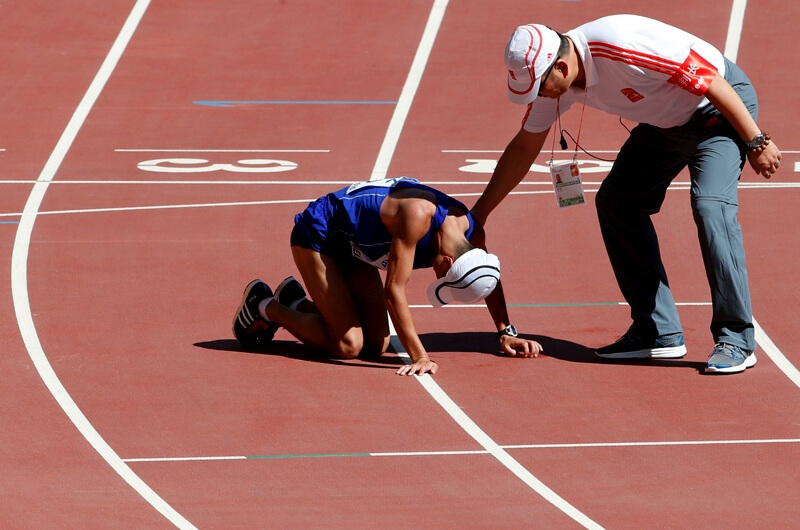
\includegraphics[width=300px]{cover} \end{center}
\newpage 
\tableofcontents 
\newpage

\newpage

\section{Problem Set}\label{problem-set}

\subsection*{1.a}\label{a}
\addcontentsline{toc}{subsection}{1.a}

\begin{Shaded}
\begin{Highlighting}[]
\FunctionTok{par}\NormalTok{(}\AttributeTok{oma =} \FunctionTok{c}\NormalTok{(}\DecValTok{3}\NormalTok{, }\DecValTok{0}\NormalTok{, }\DecValTok{2}\NormalTok{, }\DecValTok{0}\NormalTok{)) }
\FunctionTok{pairs}\NormalTok{(Bombed }\SpecialCharTok{\textasciitilde{}}\NormalTok{ . , }\AttributeTok{data=}\NormalTok{data, }\AttributeTok{pch=}\DecValTok{16}\NormalTok{, }
      \AttributeTok{col =} \FunctionTok{ifelse}\NormalTok{(data}\SpecialCharTok{$}\NormalTok{Bombed }\SpecialCharTok{==} \ConstantTok{TRUE}\NormalTok{, }\StringTok{"tomato3"}\NormalTok{, }\StringTok{"gray"}\NormalTok{), }
      \AttributeTok{main=}\StringTok{"Pairwise Relationships of Runner Features."}\NormalTok{)}

\CommentTok{\# Create a transparent, invisible plot over the entire canvas}
\FunctionTok{par}\NormalTok{(}\AttributeTok{fig =} \FunctionTok{c}\NormalTok{(}\DecValTok{0}\NormalTok{, }\DecValTok{1}\NormalTok{, }\DecValTok{0}\NormalTok{, }\DecValTok{1}\NormalTok{), }\AttributeTok{oma =} \FunctionTok{c}\NormalTok{(}\DecValTok{0}\NormalTok{, }\DecValTok{0}\NormalTok{, }\DecValTok{0}\NormalTok{, }\DecValTok{0}\NormalTok{), }\AttributeTok{mar =} \FunctionTok{c}\NormalTok{(}\DecValTok{0}\NormalTok{, }\DecValTok{0}\NormalTok{, }\DecValTok{0}\NormalTok{, }\DecValTok{0}\NormalTok{), }\AttributeTok{new =} \ConstantTok{TRUE}\NormalTok{)}
\FunctionTok{plot}\NormalTok{(}\DecValTok{0}\NormalTok{, }\DecValTok{0}\NormalTok{, }\AttributeTok{type =} \StringTok{\textquotesingle{}n\textquotesingle{}}\NormalTok{, }\AttributeTok{bty =} \StringTok{\textquotesingle{}n\textquotesingle{}}\NormalTok{, }\AttributeTok{xaxt =} \StringTok{\textquotesingle{}n\textquotesingle{}}\NormalTok{, }\AttributeTok{yaxt =} \StringTok{\textquotesingle{}n\textquotesingle{}}\NormalTok{)}

\FunctionTok{legend}\NormalTok{(}\StringTok{"bottom"}\NormalTok{, }\AttributeTok{legend =} \FunctionTok{c}\NormalTok{(}\StringTok{"Safe (FALSE)"}\NormalTok{, }\StringTok{"Bombed (TRUE)"}\NormalTok{), }
       \AttributeTok{col =} \FunctionTok{c}\NormalTok{(}\StringTok{"gray"}\NormalTok{, }\StringTok{"tomato3"}\NormalTok{), }\AttributeTok{pch =} \DecValTok{16}\NormalTok{, }
       \AttributeTok{horiz =} \ConstantTok{TRUE}\NormalTok{, }\AttributeTok{bty =} \StringTok{"n"}\NormalTok{, }\AttributeTok{inset =} \FunctionTok{c}\NormalTok{(}\DecValTok{0}\NormalTok{, }\DecValTok{0}\NormalTok{))}
\end{Highlighting}
\end{Shaded}

\begin{figure}[H]
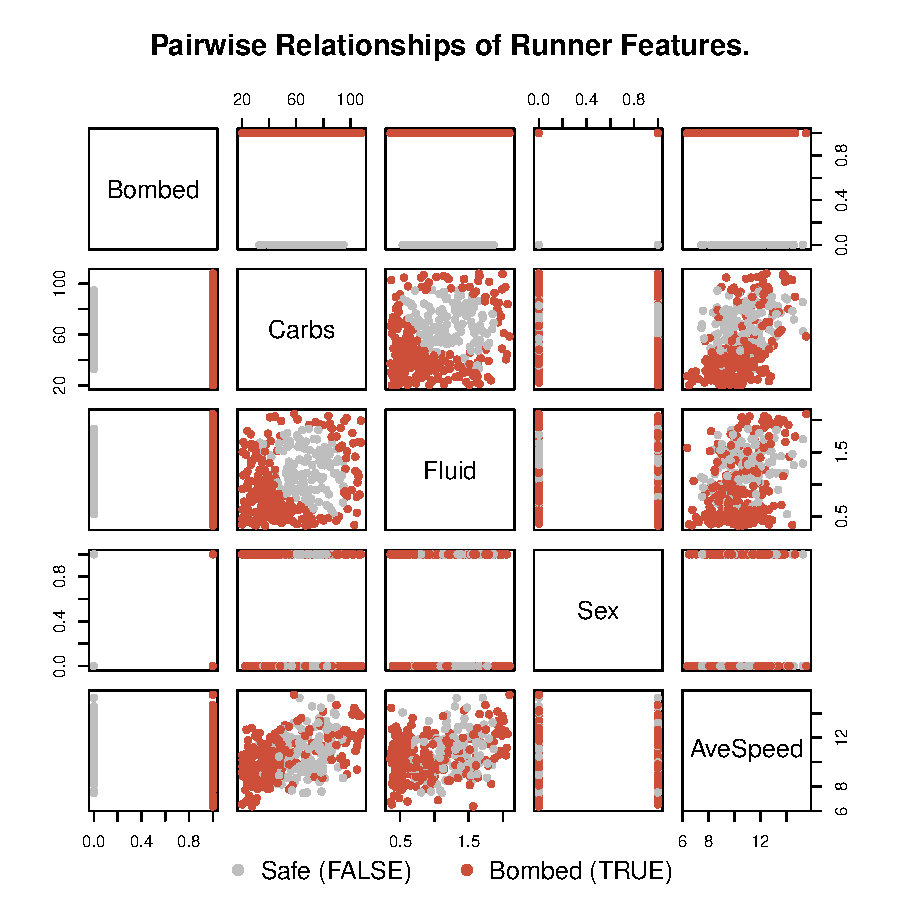
\includegraphics[width=1\linewidth]{YHXJIN001_Analytics_2026_A2_files/figure-latex/unnamed-chunk-2-1} \caption{Pairwise comparison of continuous features colored by runner outcome (black = Safe, red = Bombed). The lack of linear separability justifies the application of deep learning techniques.}\label{fig:unnamed-chunk-2}
\end{figure}

\begin{Shaded}
\begin{Highlighting}[]
\FunctionTok{par}\NormalTok{(}\AttributeTok{oma =} \FunctionTok{c}\NormalTok{(}\DecValTok{0}\NormalTok{, }\DecValTok{0}\NormalTok{, }\DecValTok{0}\NormalTok{, }\DecValTok{0}\NormalTok{), }\AttributeTok{fig =} \FunctionTok{c}\NormalTok{(}\DecValTok{0}\NormalTok{, }\DecValTok{1}\NormalTok{, }\DecValTok{0}\NormalTok{, }\DecValTok{1}\NormalTok{))}
\end{Highlighting}
\end{Shaded}

\begin{Shaded}
\begin{Highlighting}[]
\FunctionTok{par}\NormalTok{(}\AttributeTok{mfrow=}\FunctionTok{c}\NormalTok{(}\DecValTok{2}\NormalTok{,}\DecValTok{2}\NormalTok{))}


\FunctionTok{boxplot}\NormalTok{(data}\SpecialCharTok{$}\NormalTok{Carbs }\SpecialCharTok{\textasciitilde{}}\NormalTok{ data}\SpecialCharTok{$}\NormalTok{Bombed, }\AttributeTok{col=}\FunctionTok{ifelse}\NormalTok{(data}\SpecialCharTok{$}\NormalTok{Bombed }\SpecialCharTok{==} \ConstantTok{TRUE}\NormalTok{, }\StringTok{"tomato3"}\NormalTok{, }\StringTok{"gray"}\NormalTok{), }\AttributeTok{main=}\StringTok{"Boxplot of carbohydrate intake by bombed."}\NormalTok{, }
     \AttributeTok{xlab=}\StringTok{"Bombed"}\NormalTok{, }\AttributeTok{ylab=}\StringTok{"Carbohydrate intake (g/h)"}\NormalTok{,}
     \AttributeTok{cex.main =} \FloatTok{0.8}\NormalTok{,}
     \AttributeTok{names.arg =} \FunctionTok{c}\NormalTok{(}\ConstantTok{TRUE}\NormalTok{,}\ConstantTok{FALSE}\NormalTok{))}

\FunctionTok{boxplot}\NormalTok{(data}\SpecialCharTok{$}\NormalTok{Fluid }\SpecialCharTok{\textasciitilde{}}\NormalTok{ data}\SpecialCharTok{$}\NormalTok{Bombed, }\AttributeTok{col=}\FunctionTok{ifelse}\NormalTok{(data}\SpecialCharTok{$}\NormalTok{Bombed }\SpecialCharTok{==} \ConstantTok{TRUE}\NormalTok{, }\StringTok{"tomato3"}\NormalTok{, }\StringTok{"gray"}\NormalTok{), }\AttributeTok{main=}\StringTok{"Boxplot of fluid intake by bombed."}\NormalTok{, }
     \AttributeTok{xlab=}\StringTok{"Bombed"}\NormalTok{, }\AttributeTok{ylab=}\StringTok{"Fluid intake (L/h)"}\NormalTok{,}
     \AttributeTok{cex.main =} \FloatTok{0.8}\NormalTok{,}
     \AttributeTok{names.arg =} \FunctionTok{c}\NormalTok{(}\ConstantTok{TRUE}\NormalTok{,}\ConstantTok{FALSE}\NormalTok{))}

\FunctionTok{boxplot}\NormalTok{(data}\SpecialCharTok{$}\NormalTok{AveSpeed }\SpecialCharTok{\textasciitilde{}}\NormalTok{ data}\SpecialCharTok{$}\NormalTok{Bombed, }\AttributeTok{col=}\FunctionTok{ifelse}\NormalTok{(data}\SpecialCharTok{$}\NormalTok{Bombed }\SpecialCharTok{==} \ConstantTok{TRUE}\NormalTok{, }\StringTok{"tomato3"}\NormalTok{, }\StringTok{"gray"}\NormalTok{), }\AttributeTok{main=}\StringTok{"Boxplot of average speed by bombed."}\NormalTok{, }
     \AttributeTok{xlab=}\StringTok{"Bombed"}\NormalTok{, }\AttributeTok{ylab=}\StringTok{"Average speed (km/h)"}\NormalTok{,}
     \AttributeTok{cex.main =} \FloatTok{0.8}\NormalTok{,}
     \AttributeTok{names.arg =} \FunctionTok{c}\NormalTok{(}\ConstantTok{TRUE}\NormalTok{,}\ConstantTok{FALSE}\NormalTok{))}

\NormalTok{sex\_tab }\OtherTok{=} \FunctionTok{prop.table}\NormalTok{(}\FunctionTok{table}\NormalTok{(data}\SpecialCharTok{$}\NormalTok{Sex, data}\SpecialCharTok{$}\NormalTok{Bombed), }\DecValTok{1}\NormalTok{)}
\FunctionTok{rownames}\NormalTok{(sex\_tab) }\OtherTok{=} \FunctionTok{c}\NormalTok{(}\StringTok{"Female"}\NormalTok{, }\StringTok{"Male"}\NormalTok{)}
\FunctionTok{colnames}\NormalTok{(sex\_tab) }\OtherTok{=} \FunctionTok{c}\NormalTok{(}\StringTok{"FALSE"}\NormalTok{, }\StringTok{"TRUE"}\NormalTok{)}
\NormalTok{plot\_data }\OtherTok{=} \FunctionTok{t}\NormalTok{(sex\_tab)}
\FunctionTok{barplot}\NormalTok{(plot\_data, }\AttributeTok{beside=}\ConstantTok{TRUE}\NormalTok{, }\AttributeTok{ylim=}\FunctionTok{c}\NormalTok{(}\DecValTok{0}\NormalTok{, }\DecValTok{1}\NormalTok{), }\AttributeTok{xtick=}\FunctionTok{c}\NormalTok{(}\StringTok{"Bombed"}\NormalTok{, }\StringTok{"Safe"}\NormalTok{),}
        \AttributeTok{xlab=}\StringTok{"Sex"}\NormalTok{, }\AttributeTok{ylab=}\StringTok{"Proportion"}\NormalTok{,}
        \AttributeTok{main=}\StringTok{"Proportion of Runners Bombed by Sex."}\NormalTok{,}
        \AttributeTok{col=}\FunctionTok{c}\NormalTok{(}\StringTok{"gray"}\NormalTok{, }\StringTok{"tomato3"}\NormalTok{),}
        \AttributeTok{cex.main =} \FloatTok{0.8}
\NormalTok{        )}
\end{Highlighting}
\end{Shaded}

\begin{figure}[H]
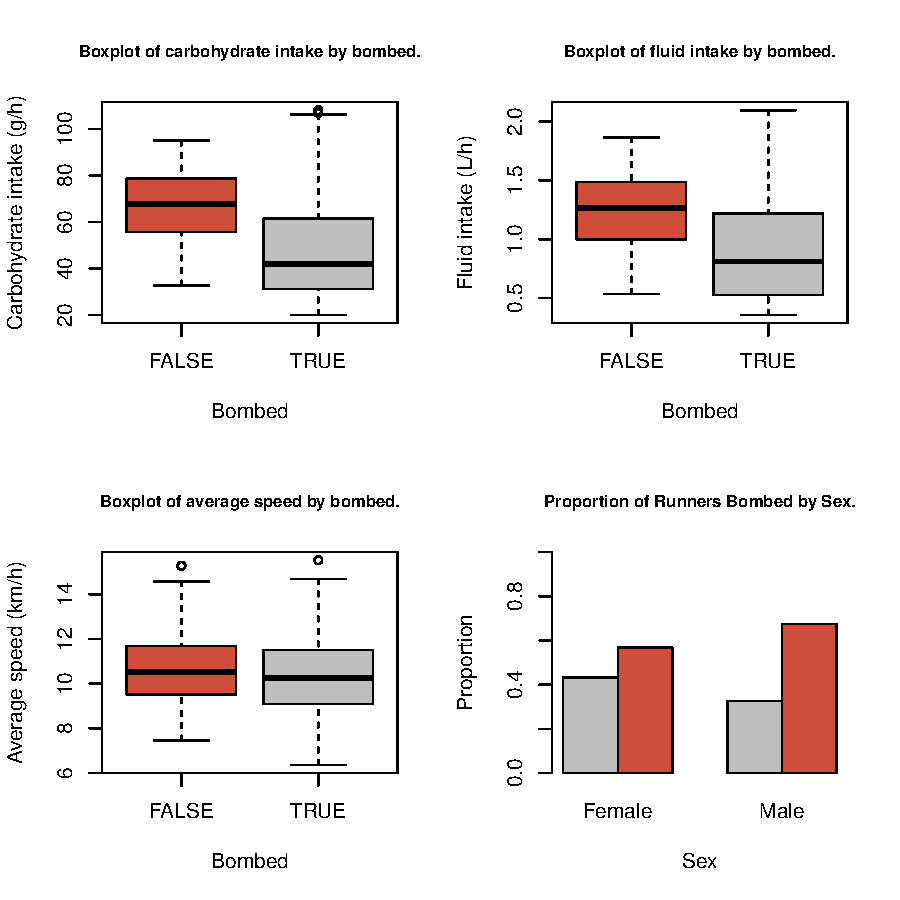
\includegraphics[width=1\linewidth]{YHXJIN001_Analytics_2026_A2_files/figure-latex/unnamed-chunk-3-1} \caption{Boxplot of average speed, carbohydrate intake hour, fluid intake per hour by bombed status and the conditional proportion of runners experiencing a 'wall' event by sex.}\label{fig:unnamed-chunk-3}
\end{figure}

\begin{Shaded}
\begin{Highlighting}[]
\FunctionTok{par}\NormalTok{(}\AttributeTok{mfrow =} \FunctionTok{c}\NormalTok{(}\DecValTok{1}\NormalTok{, }\DecValTok{1}\NormalTok{))}
\end{Highlighting}
\end{Shaded}

From the pairwise plots (Figure 1), we can see massive overlap between
the classes across every single feature. There is no clear linear
threshold in any 2D projection that separates the runners who bombed
from those who did not. This high degree of overlap and the likelihood
of complex feature interactions motivates our decision to model the
response with a neural network, which is much more flexible in modelling
non-linear, multi-dimensional boundaries. Furthermore, this is a
classification problem, which motivates our choice of using softmax as
our output layer activation function.

From the boxplots(Figure 2), we may observe that there is minimal
difference in the spread of average speed conditioned on bombed status.
On the other hand, the differences in the spread of carbohydrate and
fluid intake conditional on bombed status suggest that the distributions
differ based on bombed status.

Furthermore, from the boxplots (Figure 2), we may also see that the
features have ranges that vary greatly. This is bad for neural networks.
We would have needed to rescale the data if we were using standard
gradient descent. However, R's nlm uses a Newton-like second-order
derivative optimisation algorithm, which implicitly takes care of the
scaling.

\subsection*{1.b}\label{b}
\addcontentsline{toc}{subsection}{1.b}

We start with Equation 2:

\[
\sigma(z_j) = \frac{\exp(z_j - z^\star)}{\sum_{i=1}^q \exp(z_i - z^\star)}.
\]

Using the exponent rule \(\exp(a - b) = \exp(a)\exp(-b)\), we can expand
both the numerator and the denominator:

\[
\sigma(z_j) = \frac{\exp(z_j)\exp(-z^\star)}{\sum_{i=1}^q [\exp(z_i)\exp(-z^\star)]}.
\]

Because the term \(\exp(-z^\star)\) is a constant with respect to the
summation index \(i\), we can factor it completely out of the sum in the
denominator:

\[
\sigma(z_j) = \frac{\exp(z_j)\exp(-z^\star)}{\exp(-z^\star) \sum_{i=1}^q \exp(z_i)}.
\]

We cancel out the \(\exp(-z^\star)\) terms in the numerator and
denominator, leaving us with Equation 1:

\[
\sigma(z_j) = \frac{\exp(z_j)}{\sum_{i=1}^q \exp(z_i)}.
\]

We do this due to computational constraints. Exponential functions grow
quickly as the input value increases, but there is a limit of the number
of bits that can be used to represent a number. Hence, we subtract
\(z_j\) off the max \(z\) value to ensure that the kernel is always
negative, effectively bounding the values between 0 and 1.

\subsection*{1.c}\label{c}
\addcontentsline{toc}{subsection}{1.c}

\begin{Shaded}
\begin{Highlighting}[]
\NormalTok{softmax }\OtherTok{=} \ControlFlowTok{function}\NormalTok{(Z\_l)\{}
  \CommentTok{\# This fucntion takes in a q x N matrix,}
  \CommentTok{\# with z vector for each observation as columns}
  \CommentTok{\# Outputs a q x N probability matrix}
  
  \CommentTok{\# We first calculatethe max value for each column}
\NormalTok{  z\_max }\OtherTok{=} \FunctionTok{apply}\NormalTok{(Z\_l, }\DecValTok{2}\NormalTok{, max)}
  \CommentTok{\# turn the max matrix into a diagonal matrix}
  \CommentTok{\# Use Diagonal to prevent exp(0) = 1}
\NormalTok{  expZ\_max }\OtherTok{=} \FunctionTok{Diagonal}\NormalTok{(}\AttributeTok{x =} \FunctionTok{exp}\NormalTok{(}\SpecialCharTok{{-}}\NormalTok{z\_max))}
\NormalTok{  expZ\_l }\OtherTok{=} \FunctionTok{exp}\NormalTok{(Z\_l)}
\NormalTok{  expDiff }\OtherTok{=}\NormalTok{ expZ\_l }\SpecialCharTok{\%*\%}\NormalTok{ expZ\_max}
  
  \CommentTok{\# Get the denominators }
\NormalTok{  Denominator }\OtherTok{=} \FunctionTok{Diagonal}\NormalTok{(}\AttributeTok{x =} \DecValTok{1}\SpecialCharTok{/}\FunctionTok{colSums}\NormalTok{(expDiff))}
  
\NormalTok{  S }\OtherTok{=}\NormalTok{ expDiff }\SpecialCharTok{\%*\%}\NormalTok{ Denominator}
  \FunctionTok{return}\NormalTok{(}\FunctionTok{as.matrix}\NormalTok{(S))}
\NormalTok{\}}
\end{Highlighting}
\end{Shaded}

\subsection*{1.d}\label{d}
\addcontentsline{toc}{subsection}{1.d}

Since we are interpreting each observation as row vectors, we can safely
define the matrix \(X = [X^u X^v]_{N \times (p^u + p^v)}\). In that
case, recall that \(A_1^u = {W_1^u}^T {X^u}^T + \vec{b_1^u}\) and
\(A_1^v = {W_1^v}^TX^v + \vec{b_1^v}\), we apply the same logic and
define \(A_1 = [A_1^u A_1^v]^T_{(d^1_u + d^1_v)\times N}\). Similarly,
we define \(W_1 = \big[\begin{smallmatrix}
  W_1^u & O\\
  O & W_1^v
\end{smallmatrix}\big]_{(p^u + p^v) \times (d^1_u + d^1_v)}\) and
\(\vec{b_1} = [b_1^u b_1^v]^T\). We thus have that
\[A_1 = W_1^TX + \vec{b_1}\].

We repeat the same procedure to get \[
A_2 = \sigma(W_2^T A_1 + \vec{b_2}),
\]

\[
A_3 = \sigma_{out}(W_3^T A_2 + \vec{b_3}).
\]

\subsection*{1.e}\label{e}
\addcontentsline{toc}{subsection}{1.e}

\begin{Shaded}
\begin{Highlighting}[]
\NormalTok{Xu }\OtherTok{=} \FunctionTok{cbind}\NormalTok{(data}\SpecialCharTok{$}\NormalTok{AveSpeed, data}\SpecialCharTok{$}\NormalTok{Sex)}
\NormalTok{Xv }\OtherTok{=} \FunctionTok{cbind}\NormalTok{(data}\SpecialCharTok{$}\NormalTok{Carbs, data}\SpecialCharTok{$}\NormalTok{Fluid)}

\CommentTok{\# One{-}hot encoding the response for two outputs as requested}
\NormalTok{Y }\OtherTok{=} \FunctionTok{cbind}\NormalTok{(}\DecValTok{1} \SpecialCharTok{{-}}\NormalTok{ data}\SpecialCharTok{$}\NormalTok{Bombed, data}\SpecialCharTok{$}\NormalTok{Bombed)}
\end{Highlighting}
\end{Shaded}

\subsection*{1.f}\label{f}
\addcontentsline{toc}{subsection}{1.f}

Assume that the output layer has \(n\) nodes. The number of
\textbf{weights} is calculated per layer (\(W_1\), \(W_2\), \(W_3\)): \[
\text{Weights} = (p^u m + p^v m) + (m \times 1 + m \times 1) + (2 \times n)
\] Substituting our dataset values (\(m = 4\), \(p^u = 2\), \(p^v = 2\),
\(n = 2\)): \[
\text{Weights} = (2(4) + 2(4)) + (4 \times 1 + 4 \times 1) + (2 \times 2)
\] \[
\text{Weights} = 16 + 8 + 4 = 28
\]

The number of \textbf{biases} is calculated per layer (\(b_1\), \(b_2\),
\(b_3\)): \[
\text{Biases} = (m + m) + (1 + 1) + n
\] Substituting our dataset values: \[
\text{Biases} = (4 + 4) + 2 + 2
\] \[
\text{Biases} = 8 + 2 + 2 = 12
\] Summing the weights and biases (\(28 + 12\)), we have a total of 40
learnable parameters.

\subsection*{1.g}\label{g}
\addcontentsline{toc}{subsection}{1.g}

\begin{Shaded}
\begin{Highlighting}[]
\NormalTok{sig }\OtherTok{=} \ControlFlowTok{function}\NormalTok{(A)\{}
  \FunctionTok{return}\NormalTok{(}\FunctionTok{tanh}\NormalTok{(A))}
\NormalTok{\}}
\CommentTok{\#sig\_out = function(a)\{}
\CommentTok{\#  return (1/(1+exp({-}a)))}
\CommentTok{\#\}}
\NormalTok{sig\_out }\OtherTok{=} \ControlFlowTok{function}\NormalTok{(A)\{}
  \FunctionTok{return}\NormalTok{ (}\FunctionTok{softmax}\NormalTok{(A))}
\NormalTok{\}}

\NormalTok{obj }\OtherTok{=} \ControlFlowTok{function}\NormalTok{(Y, Y\_hat)\{}
\NormalTok{  epsilon }\OtherTok{=} \FloatTok{1e{-}8} \CommentTok{\# to prevent log(0)}
\NormalTok{  Y\_hat }\OtherTok{=} \FunctionTok{pmax}\NormalTok{(}\FunctionTok{pmin}\NormalTok{(Y\_hat, }\DecValTok{1}\SpecialCharTok{{-}}\NormalTok{epsilon),epsilon)}
  \FunctionTok{return}\NormalTok{ (}\FunctionTok{sum}\NormalTok{(}\SpecialCharTok{{-}}\NormalTok{(Y }\SpecialCharTok{*} \FunctionTok{log}\NormalTok{(Y\_hat))))}
\NormalTok{\}}

\NormalTok{neural\_net }\OtherTok{=} \ControlFlowTok{function}\NormalTok{(Xu, Xv, m, theta, nu, }\AttributeTok{Y=}\ConstantTok{NULL}\NormalTok{)\{}
  \CommentTok{\# output: Y\_hat: Raw probability output of the logistic function}
  \CommentTok{\# output: pred: prediction value}
  \CommentTok{\# output: E: evaluation error as required}
  
\NormalTok{  pu }\OtherTok{=} \FunctionTok{dim}\NormalTok{(Xu)[}\DecValTok{2}\NormalTok{]}
\NormalTok{  pv }\OtherTok{=} \FunctionTok{dim}\NormalTok{(Xv)[}\DecValTok{2}\NormalTok{]}
\NormalTok{  N }\OtherTok{=} \FunctionTok{dim}\NormalTok{(Xu)[}\DecValTok{1}\NormalTok{]}
\NormalTok{  X }\OtherTok{=} \FunctionTok{cbind}\NormalTok{(Xu, Xv)}
  
  \CommentTok{\# 1st layer (m nodes per hemisphere)}
\NormalTok{  index }\OtherTok{=} \DecValTok{1}\SpecialCharTok{:}\NormalTok{(m}\SpecialCharTok{*}\NormalTok{pu)}
\NormalTok{  W1u }\OtherTok{=} \FunctionTok{matrix}\NormalTok{(theta[index], pu, m)}
\NormalTok{  index }\OtherTok{=} \FunctionTok{max}\NormalTok{(index) }\SpecialCharTok{+} \DecValTok{1}\SpecialCharTok{:}\NormalTok{(pv}\SpecialCharTok{*}\NormalTok{m)}
\NormalTok{  W1v }\OtherTok{=} \FunctionTok{matrix}\NormalTok{(theta[index], pv, m)}
\NormalTok{  W1 }\OtherTok{=} \FunctionTok{as.matrix}\NormalTok{(}\FunctionTok{bdiag}\NormalTok{(W1u, W1v))}
  
  \CommentTok{\# 2nd layer (SPLIT BRAIN: 1 node per hemisphere)}
\NormalTok{  index }\OtherTok{=} \FunctionTok{max}\NormalTok{(index) }\SpecialCharTok{+} \DecValTok{1}\SpecialCharTok{:}\NormalTok{m}
\NormalTok{  W2u }\OtherTok{=} \FunctionTok{matrix}\NormalTok{(theta[index], m, }\DecValTok{1}\NormalTok{)}
\NormalTok{  index }\OtherTok{=} \FunctionTok{max}\NormalTok{(index) }\SpecialCharTok{+} \DecValTok{1}\SpecialCharTok{:}\NormalTok{m}
\NormalTok{  W2v }\OtherTok{=} \FunctionTok{matrix}\NormalTok{(theta[index], m, }\DecValTok{1}\NormalTok{)}
\NormalTok{  W2 }\OtherTok{=} \FunctionTok{as.matrix}\NormalTok{(}\FunctionTok{bdiag}\NormalTok{(W2u, W2v))}
  
  \CommentTok{\# Output layer (Fully connected, 4 parameters)}
\NormalTok{  index }\OtherTok{=} \FunctionTok{max}\NormalTok{(index) }\SpecialCharTok{+} \DecValTok{1}\SpecialCharTok{:}\DecValTok{4}
\NormalTok{  W3 }\OtherTok{=} \FunctionTok{matrix}\NormalTok{(theta[index], }\DecValTok{2}\NormalTok{, }\DecValTok{2}\NormalTok{)}
  
  \CommentTok{\# Biases Layer 1}
\NormalTok{  index }\OtherTok{=} \FunctionTok{max}\NormalTok{(index) }\SpecialCharTok{+} \DecValTok{1}\SpecialCharTok{:}\NormalTok{m}
\NormalTok{  b1u }\OtherTok{=} \FunctionTok{matrix}\NormalTok{(theta[index], m, }\DecValTok{1}\NormalTok{)}
\NormalTok{  index }\OtherTok{=} \FunctionTok{max}\NormalTok{(index) }\SpecialCharTok{+} \DecValTok{1}\SpecialCharTok{:}\NormalTok{m}
\NormalTok{  b1v }\OtherTok{=} \FunctionTok{matrix}\NormalTok{(theta[index], m, }\DecValTok{1}\NormalTok{)}
\NormalTok{  b1 }\OtherTok{=} \FunctionTok{rbind}\NormalTok{(b1u, b1v)}
  
  \CommentTok{\# Biases Layer 2 (1 bias per hemisphere, 2 total)}
\NormalTok{  index }\OtherTok{=} \FunctionTok{max}\NormalTok{(index) }\SpecialCharTok{+} \DecValTok{1}\SpecialCharTok{:}\DecValTok{2}
\NormalTok{  b2 }\OtherTok{=} \FunctionTok{matrix}\NormalTok{(theta[index], }\DecValTok{2}\NormalTok{, }\DecValTok{1}\NormalTok{)}
  
  \CommentTok{\# Biases Output Layer (2 nodes, 2 biases)}
\NormalTok{  index }\OtherTok{=} \FunctionTok{max}\NormalTok{(index) }\SpecialCharTok{+} \DecValTok{1}\SpecialCharTok{:}\DecValTok{2}
\NormalTok{  b3 }\OtherTok{=} \FunctionTok{matrix}\NormalTok{(theta[index], }\DecValTok{2}\NormalTok{, }\DecValTok{1}\NormalTok{)}
  
  \CommentTok{\# Forward Pass}
\NormalTok{  ones }\OtherTok{=} \FunctionTok{matrix}\NormalTok{(}\DecValTok{1}\NormalTok{, N, }\DecValTok{1}\NormalTok{)}
\NormalTok{  A0 }\OtherTok{=} \FunctionTok{as.matrix}\NormalTok{(}\FunctionTok{t}\NormalTok{(X))}
\NormalTok{  A1 }\OtherTok{=} \FunctionTok{sig}\NormalTok{(}\FunctionTok{t}\NormalTok{(W1) }\SpecialCharTok{\%*\%}\NormalTok{ A0 }\SpecialCharTok{+}\NormalTok{ b1 }\SpecialCharTok{\%*\%} \FunctionTok{t}\NormalTok{(ones))}
\NormalTok{  A2 }\OtherTok{=} \FunctionTok{sig}\NormalTok{(}\FunctionTok{t}\NormalTok{(W2) }\SpecialCharTok{\%*\%}\NormalTok{ A1 }\SpecialCharTok{+}\NormalTok{ b2 }\SpecialCharTok{\%*\%} \FunctionTok{t}\NormalTok{(ones))}
\NormalTok{  Z\_out }\OtherTok{=} \FunctionTok{t}\NormalTok{(W3) }\SpecialCharTok{\%*\%}\NormalTok{ A2 }\SpecialCharTok{+}\NormalTok{ b3 }\SpecialCharTok{\%*\%} \FunctionTok{t}\NormalTok{(ones)}
  
  \CommentTok{\# Output mapping}
\NormalTok{  Y\_hat }\OtherTok{=} \FunctionTok{t}\NormalTok{(}\FunctionTok{sig\_out}\NormalTok{(Z\_out))}
\NormalTok{  pred }\OtherTok{=} \FunctionTok{max.col}\NormalTok{(Y\_hat) }\SpecialCharTok{{-}} \DecValTok{1}
  
  \CommentTok{\# Evaluation}
\NormalTok{  E }\OtherTok{=} \ConstantTok{NULL}
  \ControlFlowTok{if}\NormalTok{ (}\SpecialCharTok{!}\FunctionTok{is.null}\NormalTok{(Y))\{}
\NormalTok{    base\_error }\OtherTok{=} \FunctionTok{obj}\NormalTok{(Y, Y\_hat) }\SpecialCharTok{/} \FunctionTok{nrow}\NormalTok{(Y)}
\NormalTok{    penalty }\OtherTok{=}\NormalTok{ (nu }\SpecialCharTok{/} \FunctionTok{nrow}\NormalTok{(Y)) }\SpecialCharTok{*}\NormalTok{ (}\FunctionTok{sum}\NormalTok{(W1}\SpecialCharTok{\^{}}\DecValTok{2}\NormalTok{) }\SpecialCharTok{+} \FunctionTok{sum}\NormalTok{(W2}\SpecialCharTok{\^{}}\DecValTok{2}\NormalTok{) }\SpecialCharTok{+} \FunctionTok{sum}\NormalTok{(W3}\SpecialCharTok{\^{}}\DecValTok{2}\NormalTok{))}
\NormalTok{    E }\OtherTok{=}\NormalTok{ base\_error }\SpecialCharTok{+}\NormalTok{ penalty}
\NormalTok{  \}}
  
  \FunctionTok{return}\NormalTok{(}\FunctionTok{list}\NormalTok{(}\AttributeTok{Y\_hat =}\NormalTok{ Y\_hat, }\AttributeTok{pred =}\NormalTok{ pred, }\AttributeTok{E =}\NormalTok{ E))}
\NormalTok{\}}
\end{Highlighting}
\end{Shaded}

\subsection*{1.h}\label{h}
\addcontentsline{toc}{subsection}{1.h}

\begin{Shaded}
\begin{Highlighting}[]
\FunctionTok{set.seed}\NormalTok{(}\DecValTok{2026}\NormalTok{)}
\NormalTok{m }\OtherTok{=} \DecValTok{4}
\NormalTok{N }\OtherTok{=} \FunctionTok{dim}\NormalTok{(Y)[}\DecValTok{1}\NormalTok{]}
\NormalTok{train\_indices }\OtherTok{=} \FunctionTok{sample}\NormalTok{(}\DecValTok{1}\SpecialCharTok{:}\NormalTok{N, }\AttributeTok{size=}\FunctionTok{round}\NormalTok{(}\FloatTok{0.8}\SpecialCharTok{*}\NormalTok{N))}

\NormalTok{Xtrain\_u }\OtherTok{=}\NormalTok{ Xu[train\_indices,]}
\NormalTok{Xtrain\_v }\OtherTok{=}\NormalTok{ Xv[train\_indices,]}
\NormalTok{Ytrain }\OtherTok{=} \FunctionTok{as.matrix}\NormalTok{(Y[train\_indices, ])}
     
\NormalTok{Xvalid\_u }\OtherTok{=}\NormalTok{ Xu[}\SpecialCharTok{{-}}\NormalTok{train\_indices,]}
\NormalTok{Xvalid\_v }\OtherTok{=}\NormalTok{ Xv[}\SpecialCharTok{{-}}\NormalTok{train\_indices,]}
\NormalTok{Yvalid }\OtherTok{=} \FunctionTok{as.matrix}\NormalTok{(Y[}\SpecialCharTok{{-}}\NormalTok{train\_indices, ])}

\NormalTok{pu }\OtherTok{=} \FunctionTok{dim}\NormalTok{(Xu)[}\DecValTok{2}\NormalTok{]}
\NormalTok{pv }\OtherTok{=} \FunctionTok{dim}\NormalTok{(Xv)[}\DecValTok{2}\NormalTok{]}
\NormalTok{nparams }\OtherTok{=}\NormalTok{ (pu }\SpecialCharTok{*}\NormalTok{ m) }\SpecialCharTok{+}\NormalTok{ (pv }\SpecialCharTok{*}\NormalTok{ m) }\SpecialCharTok{+} \DecValTok{2} \SpecialCharTok{*}\NormalTok{ m  }\SpecialCharTok{+} \DecValTok{2} \SpecialCharTok{*}\NormalTok{ m }\SpecialCharTok{+} \DecValTok{4} \SpecialCharTok{+} \DecValTok{4}
\NormalTok{theta }\OtherTok{=} \FunctionTok{runif}\NormalTok{(nparams, }\SpecialCharTok{{-}}\DecValTok{1}\NormalTok{, }\DecValTok{1}\NormalTok{)}

\NormalTok{nu\_grid }\OtherTok{=} \FunctionTok{exp}\NormalTok{(}\FunctionTok{seq}\NormalTok{(}\SpecialCharTok{{-}}\DecValTok{6}\NormalTok{,}\DecValTok{2}\NormalTok{,length}
            \OtherTok{=}\DecValTok{30}\NormalTok{))}
\CommentTok{\# Do grid search on values of nu\_grid}
\NormalTok{errors }\OtherTok{=} \FunctionTok{rep}\NormalTok{(}\DecValTok{1}\NormalTok{, }\FunctionTok{length}\NormalTok{(nu\_grid))}
\NormalTok{theta\_store }\OtherTok{=} \FunctionTok{matrix}\NormalTok{(}\ConstantTok{NA}\NormalTok{, }\FunctionTok{length}\NormalTok{(nu\_grid), nparams)}
\ControlFlowTok{for}\NormalTok{ (i }\ControlFlowTok{in} \DecValTok{1}\SpecialCharTok{:}\FunctionTok{length}\NormalTok{(nu\_grid))\{}
\NormalTok{  nu }\OtherTok{=}\NormalTok{ nu\_grid[i]}
  
\NormalTok{  obj\_train }\OtherTok{=} \ControlFlowTok{function}\NormalTok{(theta\_init) \{}
\NormalTok{    result }\OtherTok{=} \FunctionTok{neural\_net}\NormalTok{(Xtrain\_u, Xtrain\_v, }\DecValTok{4}\NormalTok{, theta\_init, nu, Ytrain)}
    \FunctionTok{return}\NormalTok{(result}\SpecialCharTok{$}\NormalTok{E)}
\NormalTok{  \}}
  \FunctionTok{cat}\NormalTok{(}\StringTok{"Training network for nu ="}\NormalTok{, nu, }\StringTok{"}\SpecialCharTok{\textbackslash{}n}\StringTok{"}\NormalTok{)}
\NormalTok{  trained }\OtherTok{=} \FunctionTok{nlm}\NormalTok{(obj\_train, theta, }\AttributeTok{iterlim=}\DecValTok{1000}\NormalTok{)}
\NormalTok{  theta\_store[i, ] }\OtherTok{=}\NormalTok{trained}\SpecialCharTok{$}\NormalTok{estimate}
\NormalTok{  valid\_result }\OtherTok{=} \FunctionTok{neural\_net}\NormalTok{(Xvalid\_u, Xvalid\_v, }\DecValTok{4}\NormalTok{, trained}\SpecialCharTok{$}\NormalTok{estimate, nu)}

  \FunctionTok{cat}\NormalTok{(}\StringTok{"Finished validating nu ="}\NormalTok{, nu, }\StringTok{"}\SpecialCharTok{\textbackslash{}n}\StringTok{"}\NormalTok{)}
\NormalTok{  errors[i] }\OtherTok{=} \FunctionTok{obj}\NormalTok{(Yvalid, valid\_result}\SpecialCharTok{$}\NormalTok{Y\_hat) }\SpecialCharTok{/} \FunctionTok{nrow}\NormalTok{(Xvalid\_u)}
\NormalTok{\}}
\end{Highlighting}
\end{Shaded}

\begin{figure}[H]
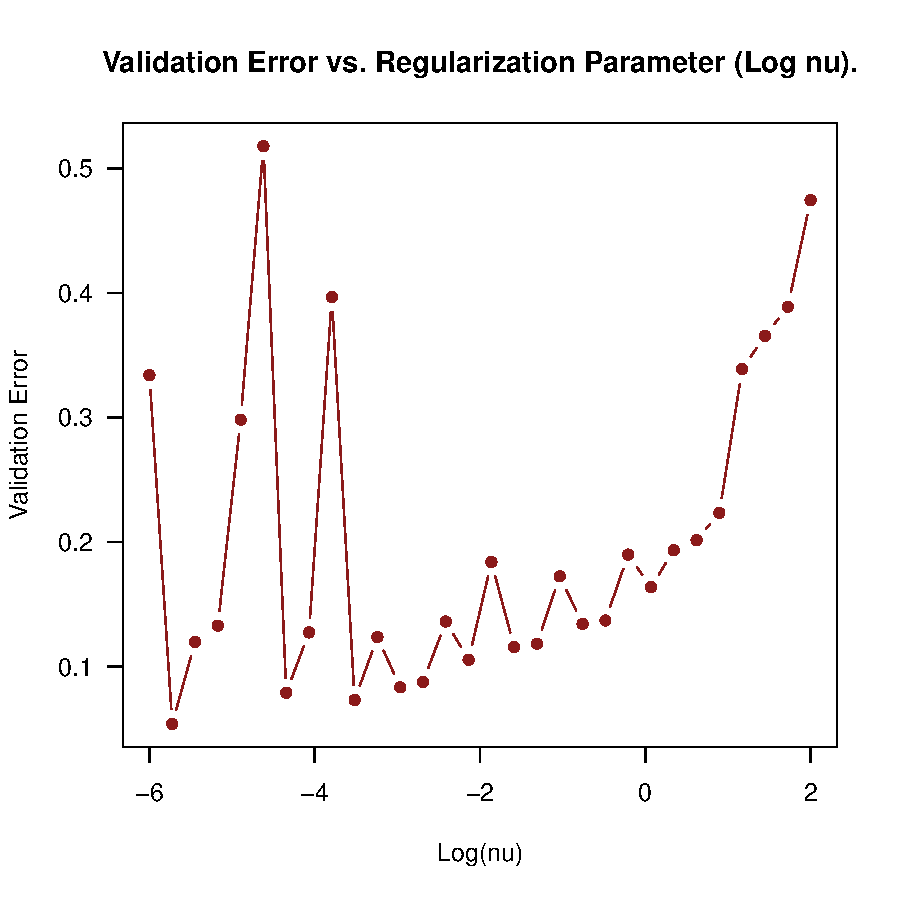
\includegraphics[width=1\linewidth]{YHXJIN001_Analytics_2026_A2_files/figure-latex/unnamed-chunk-8-1} \caption{L2 regularised cross entropy loss conditioned on L2 regularisation parameter, nu.}\label{fig:unnamed-chunk-8}
\end{figure}

From the above, the best \(\nu\) value that results in the lowest
validation loss is approximately 0.03.

\subsection*{1.i}\label{i}
\addcontentsline{toc}{subsection}{1.i}

\begin{Shaded}
\begin{Highlighting}[]
\FunctionTok{library}\NormalTok{(colorspace)}
\NormalTok{color.gradient }\OtherTok{=} \ControlFlowTok{function}\NormalTok{(x, }\AttributeTok{colors=}\FunctionTok{c}\NormalTok{(}\StringTok{\textquotesingle{}coral\textquotesingle{}}\NormalTok{,}\StringTok{\textquotesingle{}purple\textquotesingle{}}\NormalTok{,}\StringTok{\textquotesingle{}skyblue1\textquotesingle{}}\NormalTok{), }\AttributeTok{colsteps=}\DecValTok{25}\NormalTok{)}
\NormalTok{\{}
\NormalTok{  colpal }\OtherTok{=} \FunctionTok{colorRampPalette}\NormalTok{(colors)}
  \FunctionTok{return}\NormalTok{( }\FunctionTok{colpal}\NormalTok{(colsteps)[ }\FunctionTok{findInterval}\NormalTok{(x, }\FunctionTok{seq}\NormalTok{(}\FunctionTok{min}\NormalTok{(x),}\FunctionTok{max}\NormalTok{(x), }\AttributeTok{length=}\NormalTok{colsteps)) ] )}
\NormalTok{\}}


\NormalTok{M}\OtherTok{=}\DecValTok{100}
\NormalTok{carbs\_seq }\OtherTok{=} \FunctionTok{seq}\NormalTok{(}\FunctionTok{min}\NormalTok{(data}\SpecialCharTok{$}\NormalTok{Carbs),}\FunctionTok{max}\NormalTok{(data}\SpecialCharTok{$}\NormalTok{Carbs),}\AttributeTok{length.out=}\NormalTok{ M)}
\NormalTok{carbs\_mean }\OtherTok{=} \FunctionTok{mean}\NormalTok{(data}\SpecialCharTok{$}\NormalTok{Carbs)}
\NormalTok{fluid\_seq }\OtherTok{=} \FunctionTok{seq}\NormalTok{(}\FunctionTok{min}\NormalTok{(data}\SpecialCharTok{$}\NormalTok{Fluid),}\FunctionTok{max}\NormalTok{(data}\SpecialCharTok{$}\NormalTok{Fluid),}\AttributeTok{length.out=}\NormalTok{ M)}
\NormalTok{fluid\_mean }\OtherTok{=} \FunctionTok{mean}\NormalTok{(data}\SpecialCharTok{$}\NormalTok{Fluid)}

\NormalTok{xxv1 }\OtherTok{=} \FunctionTok{rep}\NormalTok{(carbs\_seq, M)}
\NormalTok{xxv2 }\OtherTok{=} \FunctionTok{rep}\NormalTok{(fluid\_seq, }\AttributeTok{each =}\NormalTok{M)}
\NormalTok{XXv }\OtherTok{=} \FunctionTok{cbind}\NormalTok{(xxv1, xxv2)}

\NormalTok{xxu1 }\OtherTok{=} \FunctionTok{rep}\NormalTok{(}\DecValTok{12}\NormalTok{, M}\SpecialCharTok{\^{}}\DecValTok{2}\NormalTok{)}
\NormalTok{xxu2\_male }\OtherTok{=} \FunctionTok{rep}\NormalTok{(}\DecValTok{1}\NormalTok{, }\AttributeTok{each =}\NormalTok{ M}\SpecialCharTok{\^{}}\DecValTok{2}\NormalTok{)}
\NormalTok{xxu2\_female }\OtherTok{=} \FunctionTok{rep}\NormalTok{(}\DecValTok{0}\NormalTok{, }\AttributeTok{each=}\NormalTok{M}\SpecialCharTok{\^{}}\DecValTok{2}\NormalTok{)}
\NormalTok{XXumale }\OtherTok{=} \FunctionTok{cbind}\NormalTok{(xxu1, xxu2\_male)}
\NormalTok{XXufemale }\OtherTok{=} \FunctionTok{cbind}\NormalTok{(xxu1, xxu2\_female)}

\NormalTok{response\_male }\OtherTok{=} \FunctionTok{neural\_net}\NormalTok{(XXumale, XXv, }\DecValTok{4}\NormalTok{, theta\_best\_nu, }\DecValTok{0}\NormalTok{)}
\NormalTok{response\_female }\OtherTok{=} \FunctionTok{neural\_net}\NormalTok{(XXufemale, XXv, }\DecValTok{4}\NormalTok{, theta\_best\_nu, }\DecValTok{0}\NormalTok{)}

\FunctionTok{plot}\NormalTok{(xxv2 }\SpecialCharTok{\textasciitilde{}}\NormalTok{ xxv1, }\AttributeTok{col=}\FunctionTok{color.gradient}\NormalTok{(response\_female}\SpecialCharTok{$}\NormalTok{Y\_hat[,}\DecValTok{2}\NormalTok{]), }\AttributeTok{pch=}\DecValTok{16}\NormalTok{, }\AttributeTok{cex=}\FloatTok{0.8}\NormalTok{, }
     \AttributeTok{xlab=}\StringTok{"Carbohydrate intake (gram/hour)"}\NormalTok{, }\AttributeTok{ylab=}\StringTok{"Fluid intake (litre/hour)"}\NormalTok{, }
     \AttributeTok{main=}\StringTok{"Female: probability of hitting the wall."}\NormalTok{)}
\FunctionTok{legend}\NormalTok{(}\StringTok{"topright"}\NormalTok{, }\AttributeTok{title=}\StringTok{"Risk of Bombing"}\NormalTok{,}
       \AttributeTok{legend=}\FunctionTok{c}\NormalTok{(}\StringTok{"High (Near 100\%)"}\NormalTok{, }\StringTok{"Medium (\textasciitilde{}50\%)"}\NormalTok{, }\StringTok{"Low (Near 0\%)"}\NormalTok{), }
       \AttributeTok{col=}\FunctionTok{c}\NormalTok{(}\StringTok{"skyblue1"}\NormalTok{, }\StringTok{"purple"}\NormalTok{, }\StringTok{"coral"}\NormalTok{), }\AttributeTok{pch=}\DecValTok{16}\NormalTok{, }\AttributeTok{bg=}\StringTok{"white"}\NormalTok{, }\AttributeTok{cex=}\FloatTok{0.7}\NormalTok{)}
\end{Highlighting}
\end{Shaded}

\begin{figure}[H]
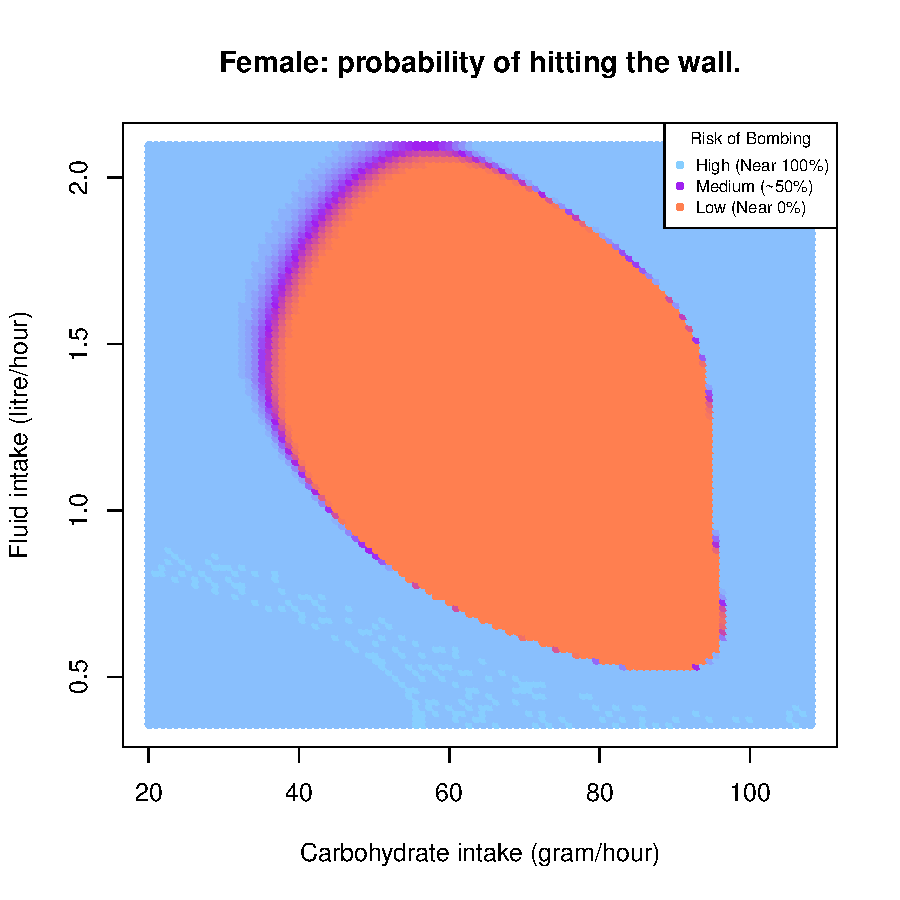
\includegraphics[width=1\linewidth]{YHXJIN001_Analytics_2026_A2_files/figure-latex/unnamed-chunk-9-1} \caption{Response plots for runners of both sexes maintaining an average speed of 12km/h according to their carbohydrate intake and fluid intake.}\label{fig:unnamed-chunk-9-1}
\end{figure}

\begin{Shaded}
\begin{Highlighting}[]
\FunctionTok{plot}\NormalTok{(xxv2 }\SpecialCharTok{\textasciitilde{}}\NormalTok{ xxv1, }\AttributeTok{col=}\FunctionTok{color.gradient}\NormalTok{(response\_male}\SpecialCharTok{$}\NormalTok{Y\_hat[,}\DecValTok{2}\NormalTok{]), }\AttributeTok{pch=}\DecValTok{16}\NormalTok{, }\AttributeTok{cex=}\FloatTok{0.8}\NormalTok{, }
     \AttributeTok{xlab=}\StringTok{"Carbohydrate intake (gram/hour)"}\NormalTok{, }\AttributeTok{ylab=}\StringTok{"Fluid intake (litre/hour)"}\NormalTok{, }
     \AttributeTok{main=}\StringTok{"Male: probability of hitting the wall."}\NormalTok{)}
\FunctionTok{legend}\NormalTok{(}\StringTok{"topright"}\NormalTok{, }\AttributeTok{title=}\StringTok{"Risk of Bombing"}\NormalTok{,}
       \AttributeTok{legend=}\FunctionTok{c}\NormalTok{(}\StringTok{"High (Near 100\%)"}\NormalTok{, }\StringTok{"Medium (\textasciitilde{}50\%)"}\NormalTok{, }\StringTok{"Low (Near 0\%)"}\NormalTok{), }
       \AttributeTok{col=}\FunctionTok{c}\NormalTok{(}\StringTok{"skyblue1"}\NormalTok{, }\StringTok{"purple"}\NormalTok{, }\StringTok{"coral"}\NormalTok{), }\AttributeTok{pch=}\DecValTok{16}\NormalTok{, }\AttributeTok{bg=}\StringTok{"white"}\NormalTok{, }\AttributeTok{cex=}\FloatTok{0.7}\NormalTok{)}
\end{Highlighting}
\end{Shaded}

\begin{figure}[H]
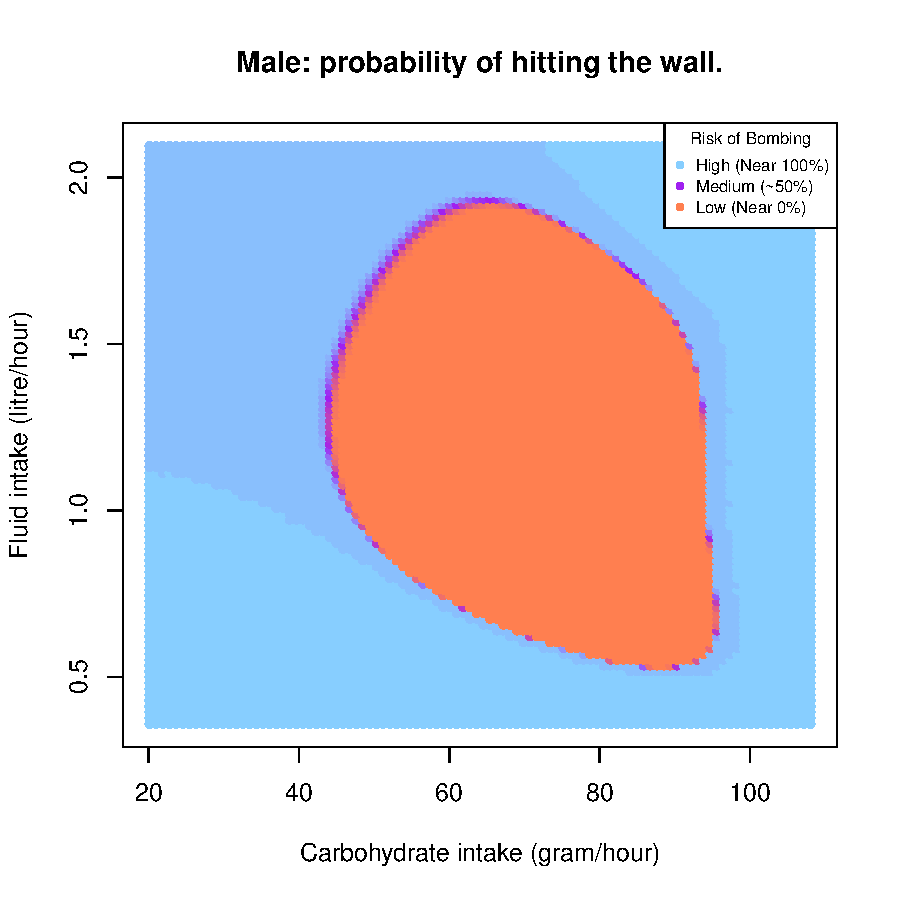
\includegraphics[width=1\linewidth]{YHXJIN001_Analytics_2026_A2_files/figure-latex/unnamed-chunk-9-2} \caption{Response plots for runners of both sexes maintaining an average speed of 12km/h according to their carbohydrate intake and fluid intake.}\label{fig:unnamed-chunk-9-2}
\end{figure}

\subsection*{1.j}\label{j}
\addcontentsline{toc}{subsection}{1.j}

From the response plots, we observe that male runners are more likely to
hit the wall running at 12km/h if they are not careful with their diet.
The safe region is fairly centred, but we may observe a negative trend:
the more carbohydrates consumed, the less fluid is needed to remain
safe, and vice versa. There is also the risk of over-consumption and
under-consumption in either category. For fluid intake, anything under
0.5 L/h and more than 2 L/h leads to a high risk of bombing. For
carbohydrate intake, the lower bound and the upper bound are 40 g/h and
100 g/h respectively.

Female runners, on the other hand, have a significantly larger safety
range compared to male athletes. Notably, females can sometimes avoid
hitting the wall even at very low carbohydrate intakes (20-40g/h)
provided their fluid intake is high (\textgreater1.5 L/h). As mentioned,
this is a physiological tolerance that males do not share. However, the
lower bound for fluid intake and the upper bound for carbohydrate intake
remain the same as male runners.

To summarise, both plots indicate a ceiling effect where over-consuming
both fluids and carbohydrates (the top-right region) increases the risk
of bombing. As such, while females have more leeway, the safest region
for both sexes running at 12km/h remains 1 L/h to 1.5 L/h of fluid and
50g/h to 90g/h of carbohydrates. This is a practical recommendation that
we advise runners of both sexes to adhere to, assuming an average
running speed of 12km/h.

\subsection*{1.k}\label{k}
\addcontentsline{toc}{subsection}{1.k}

\begin{Shaded}
\begin{Highlighting}[]
\CommentTok{\# Empirical comparison 4{-}4 network}

\NormalTok{std\_neural\_net }\OtherTok{=} \ControlFlowTok{function}\NormalTok{(X, m, theta, nu, }\AttributeTok{Y=}\ConstantTok{NULL}\NormalTok{)\{}
\NormalTok{  p }\OtherTok{=} \FunctionTok{dim}\NormalTok{(X)[}\DecValTok{2}\NormalTok{]}
\NormalTok{  N }\OtherTok{=} \FunctionTok{dim}\NormalTok{(X)[}\DecValTok{1}\NormalTok{]}
\NormalTok{  q }\OtherTok{=} \DecValTok{2}
  
\NormalTok{  index }\OtherTok{=} \DecValTok{1}\SpecialCharTok{:}\NormalTok{(m}\SpecialCharTok{*}\NormalTok{p)}
\NormalTok{  W1 }\OtherTok{=} \FunctionTok{matrix}\NormalTok{(theta[index], p, m)}
\NormalTok{  index }\OtherTok{=} \FunctionTok{max}\NormalTok{(index) }\SpecialCharTok{+} \DecValTok{1}\SpecialCharTok{:}\NormalTok{(m}\SpecialCharTok{*}\NormalTok{m)}
\NormalTok{  W2 }\OtherTok{=} \FunctionTok{matrix}\NormalTok{(theta[index], m, m)}
\NormalTok{  index }\OtherTok{=} \FunctionTok{max}\NormalTok{(index) }\SpecialCharTok{+} \DecValTok{1}\SpecialCharTok{:}\NormalTok{(m}\SpecialCharTok{*}\NormalTok{q)}
\NormalTok{  W3 }\OtherTok{=} \FunctionTok{matrix}\NormalTok{(theta[index], m, q)}
  
\NormalTok{  index }\OtherTok{=} \FunctionTok{max}\NormalTok{(index) }\SpecialCharTok{+} \DecValTok{1}\SpecialCharTok{:}\NormalTok{m}
\NormalTok{  b1 }\OtherTok{=} \FunctionTok{matrix}\NormalTok{(theta[index], m, }\DecValTok{1}\NormalTok{)}
\NormalTok{  index }\OtherTok{=} \FunctionTok{max}\NormalTok{(index) }\SpecialCharTok{+} \DecValTok{1}\SpecialCharTok{:}\NormalTok{m}
\NormalTok{  b2 }\OtherTok{=} \FunctionTok{matrix}\NormalTok{(theta[index], m, }\DecValTok{1}\NormalTok{)}
\NormalTok{  index }\OtherTok{=} \FunctionTok{max}\NormalTok{(index) }\SpecialCharTok{+} \DecValTok{1}\SpecialCharTok{:}\NormalTok{q}
\NormalTok{  b3 }\OtherTok{=} \FunctionTok{matrix}\NormalTok{(theta[index], q, }\DecValTok{1}\NormalTok{)}
  
\NormalTok{  ones }\OtherTok{=} \FunctionTok{matrix}\NormalTok{(}\DecValTok{1}\NormalTok{, N, }\DecValTok{1}\NormalTok{)}
\NormalTok{  A0 }\OtherTok{=} \FunctionTok{as.matrix}\NormalTok{(}\FunctionTok{t}\NormalTok{(X))}
\NormalTok{  A1 }\OtherTok{=} \FunctionTok{sig}\NormalTok{(}\FunctionTok{t}\NormalTok{(W1) }\SpecialCharTok{\%*\%}\NormalTok{ A0 }\SpecialCharTok{+}\NormalTok{ b1 }\SpecialCharTok{\%*\%} \FunctionTok{t}\NormalTok{(ones))}
\NormalTok{  A2 }\OtherTok{=} \FunctionTok{sig}\NormalTok{(}\FunctionTok{t}\NormalTok{(W2) }\SpecialCharTok{\%*\%}\NormalTok{ A1 }\SpecialCharTok{+}\NormalTok{ b2 }\SpecialCharTok{\%*\%} \FunctionTok{t}\NormalTok{(ones))}
\NormalTok{  Z\_out }\OtherTok{=} \FunctionTok{t}\NormalTok{(W3) }\SpecialCharTok{\%*\%}\NormalTok{ A2 }\SpecialCharTok{+}\NormalTok{ b3 }\SpecialCharTok{\%*\%} \FunctionTok{t}\NormalTok{(ones)}
  
\NormalTok{  Y\_hat }\OtherTok{=} \FunctionTok{t}\NormalTok{(}\FunctionTok{sig\_out}\NormalTok{(Z\_out))}
\NormalTok{  pred }\OtherTok{=} \FunctionTok{max.col}\NormalTok{(Y\_hat) }\SpecialCharTok{{-}} \DecValTok{1}
  
\NormalTok{  E }\OtherTok{=} \ConstantTok{NULL}
  \ControlFlowTok{if}\NormalTok{ (}\SpecialCharTok{!}\FunctionTok{is.null}\NormalTok{(Y))\{}
\NormalTok{    base\_error }\OtherTok{=} \FunctionTok{obj}\NormalTok{(Y, Y\_hat) }\SpecialCharTok{/} \FunctionTok{nrow}\NormalTok{(Y)}
\NormalTok{    penalty }\OtherTok{=}\NormalTok{ (nu }\SpecialCharTok{/} \FunctionTok{nrow}\NormalTok{(Y)) }\SpecialCharTok{*}\NormalTok{ (}\FunctionTok{sum}\NormalTok{(W1}\SpecialCharTok{\^{}}\DecValTok{2}\NormalTok{) }\SpecialCharTok{+} \FunctionTok{sum}\NormalTok{(W2}\SpecialCharTok{\^{}}\DecValTok{2}\NormalTok{) }\SpecialCharTok{+} \FunctionTok{sum}\NormalTok{(W3}\SpecialCharTok{\^{}}\DecValTok{2}\NormalTok{))}
\NormalTok{    E }\OtherTok{=}\NormalTok{ base\_error }\SpecialCharTok{+}\NormalTok{ penalty}
\NormalTok{  \}}
  \FunctionTok{return}\NormalTok{(}\FunctionTok{list}\NormalTok{(}\AttributeTok{Y\_hat =}\NormalTok{ Y\_hat, }\AttributeTok{pred =}\NormalTok{ pred, }\AttributeTok{E =}\NormalTok{ E))}
\NormalTok{\}}

\CommentTok{\# Setup the combined data}
\NormalTok{Xtrain\_full }\OtherTok{=} \FunctionTok{cbind}\NormalTok{(Xtrain\_u, Xtrain\_v)}
\NormalTok{Xvalid\_full }\OtherTok{=} \FunctionTok{cbind}\NormalTok{(Xvalid\_u, Xvalid\_v)}

\CommentTok{\# Standard (4,4) has exactly 50 parameters}
\NormalTok{std\_nparams }\OtherTok{=} \DecValTok{50} 
\FunctionTok{set.seed}\NormalTok{(}\DecValTok{2026}\NormalTok{)}
\NormalTok{std\_theta }\OtherTok{=} \FunctionTok{runif}\NormalTok{(std\_nparams, }\SpecialCharTok{{-}}\DecValTok{1}\NormalTok{, }\DecValTok{1}\NormalTok{)}
\NormalTok{std\_errors }\OtherTok{=} \FunctionTok{rep}\NormalTok{(}\DecValTok{1}\NormalTok{, }\FunctionTok{length}\NormalTok{(nu\_grid))}

\FunctionTok{cat}\NormalTok{(}\StringTok{"}\SpecialCharTok{\textbackslash{}n}\StringTok{{-}{-}{-} Training Standard Network {-}{-}{-}}\SpecialCharTok{\textbackslash{}n}\StringTok{"}\NormalTok{)}
\end{Highlighting}
\end{Shaded}

\begin{verbatim}
## 
## --- Training Standard Network ---
\end{verbatim}

\begin{Shaded}
\begin{Highlighting}[]
\ControlFlowTok{for}\NormalTok{ (i }\ControlFlowTok{in} \DecValTok{1}\SpecialCharTok{:}\FunctionTok{length}\NormalTok{(nu\_grid))\{}
\NormalTok{  nu }\OtherTok{=}\NormalTok{ nu\_grid[i]}
\NormalTok{  std\_obj\_train }\OtherTok{=} \ControlFlowTok{function}\NormalTok{(theta\_init) \{}
\NormalTok{    result }\OtherTok{=} \FunctionTok{std\_neural\_net}\NormalTok{(Xtrain\_full, }\DecValTok{4}\NormalTok{, theta\_init, nu, Ytrain)}
    \FunctionTok{return}\NormalTok{(result}\SpecialCharTok{$}\NormalTok{E)}
\NormalTok{  \}}
\NormalTok{  std\_trained }\OtherTok{=} \FunctionTok{nlm}\NormalTok{(std\_obj\_train, std\_theta, }\AttributeTok{iterlim=}\DecValTok{1000}\NormalTok{)}
\NormalTok{  std\_valid\_result }\OtherTok{=} \FunctionTok{std\_neural\_net}\NormalTok{(Xvalid\_full, }\DecValTok{4}\NormalTok{, std\_trained}\SpecialCharTok{$}\NormalTok{estimate, nu)}
\NormalTok{  std\_errors[i] }\OtherTok{=} \FunctionTok{obj}\NormalTok{(Yvalid, std\_valid\_result}\SpecialCharTok{$}\NormalTok{Y\_hat) }\SpecialCharTok{/} \FunctionTok{nrow}\NormalTok{(Xvalid\_full)}
\NormalTok{\}}

\CommentTok{\# Plot them together}
\FunctionTok{plot}\NormalTok{(}\FunctionTok{log}\NormalTok{(nu\_grid), errors, }\AttributeTok{type=}\StringTok{"b"}\NormalTok{, }\AttributeTok{col=}\StringTok{"firebrick4"}\NormalTok{, }\AttributeTok{pch=}\DecValTok{16}\NormalTok{, }
     \AttributeTok{main=}\StringTok{"Split{-}Brain vs Standard (4,4) Network"}\NormalTok{,}
     \AttributeTok{xlab=}\StringTok{"Log(nu)"}\NormalTok{, }\AttributeTok{ylab=}\StringTok{"Validation Error"}\NormalTok{, }\AttributeTok{ylim=}\FunctionTok{range}\NormalTok{(}\FunctionTok{c}\NormalTok{(errors, std\_errors)))}
\FunctionTok{lines}\NormalTok{(}\FunctionTok{log}\NormalTok{(nu\_grid), std\_errors, }\AttributeTok{type=}\StringTok{"b"}\NormalTok{, }\AttributeTok{col=}\StringTok{"skyblue"}\NormalTok{, }\AttributeTok{pch=}\DecValTok{16}\NormalTok{)}
\FunctionTok{legend}\NormalTok{(}\StringTok{"topleft"}\NormalTok{, }\AttributeTok{legend=}\FunctionTok{c}\NormalTok{(}\StringTok{"Split{-}Brain (40 params)"}\NormalTok{, }\StringTok{"Standard (50 params)"}\NormalTok{), }
       \AttributeTok{col=}\FunctionTok{c}\NormalTok{(}\StringTok{"firebrick4"}\NormalTok{, }\StringTok{"skyblue"}\NormalTok{), }\AttributeTok{lty=}\DecValTok{1}\NormalTok{, }\AttributeTok{pch=}\DecValTok{16}\NormalTok{)}
\end{Highlighting}
\end{Shaded}

\begin{figure}[H]
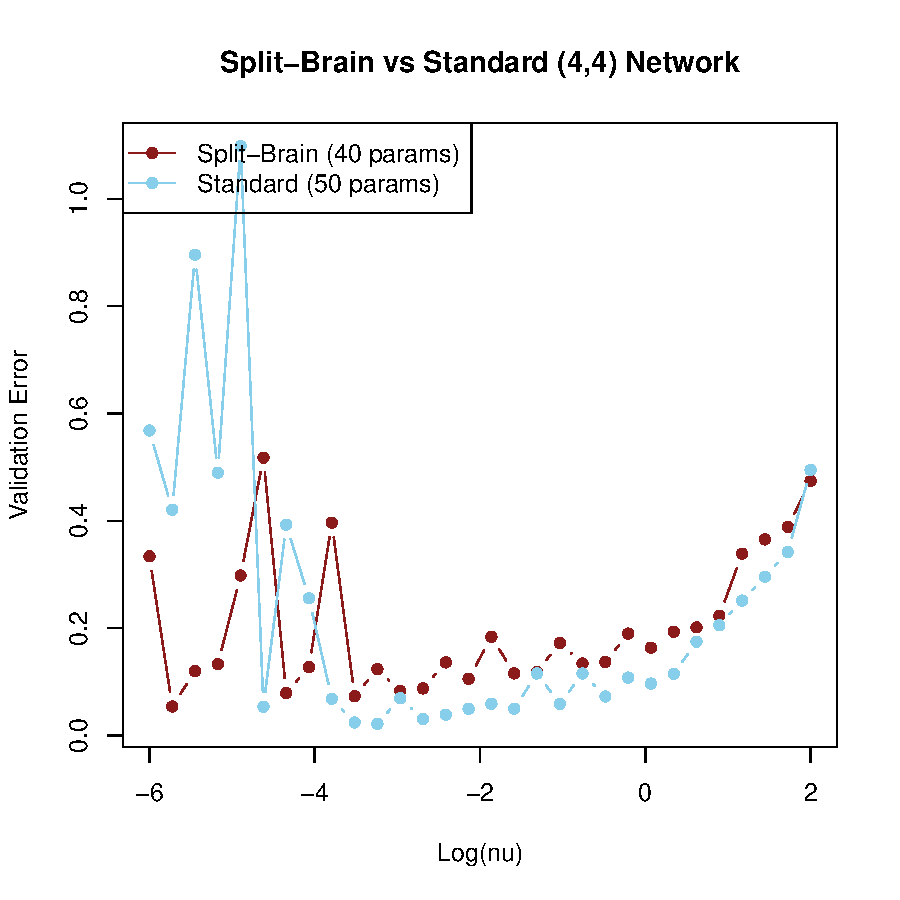
\includegraphics[width=1\linewidth]{YHXJIN001_Analytics_2026_A2_files/figure-latex/unnamed-chunk-10-1} \caption{L2 regularised cross entropy loss conditioned on L2 regularisation parameter, nu, for both the split-brain network and a regular 4, 4 neural network.}\label{fig:unnamed-chunk-10}
\end{figure}

Based on the comparative analysis, there is no empirical advantage to
using the split-brain network for modelling this specific dataset.

As demonstrated in the validation cross-entropy plot, the standard (4,4)
network consistently outperforms the split-brain network across almost
the entire grid of regularisation parameters (\nu), ultimately achieving
a lower minimum validation error.

Empirically, the data suggests that forcing the network to keep the
physiological inputs (Carbs/Fluid) and demographic inputs (Sex/Speed)
independent until the final layer creates an artificial bottleneck that
hinders performance. The standard network allows all inputs to interact
immediately in the first hidden layer. Because a runner's optimal
nutritional intake is dependent on their biological sex (as seen in our
EDA and response surfaces), allowing these features to cross-communicate
early and often yields empirically better predictions.

Furthermore, the standard (4,4) network benefits from a larger parameter
capacity (50 parameters compared to the split-brain's 40). While the
split-brain architecture offers theoretical advantages in terms of
interpretability and structural regularisation, the empirical evidence
strictly favours the standard fully-connected network for minimising
predictive error on this dataset.






\end{document}
